\documentclass[12pt,dvipdfmx]{beamer}
\usepackage{pgfpages}
\usepackage{graphicx}
\DeclareGraphicsExtensions{.eps}
\usepackage{listings,jlisting}
\usepackage{fancybox}
\usepackage{hyperref}
\usepackage{multirow}

\newif\ifja
\newif\ifeng
\jafalse
\engtrue

%%%%%%%%%%%%%%%%%%%%%%%%%%%
%%% themes
%%%%%%%%%%%%%%%%%%%%%%%%%%%
\usetheme{Boadilla}
%% no navigation bar
% default boxes Bergen Boadilla Madrid Pittsburgh Rochester
%% tree-like navigation bar
% Antibes JuanLesPins Montpellier
%% toc sidebar
% Berkeley PaloAlto Goettingen Marburg Hannover Berlin Ilmenau Dresden Darmstadt Frankfurt Singapore Szeged
%% Section and Subsection Tables
% Copenhagen Luebeck Malmoe Warsaw

%%%%%%%%%%%%%%%%%%%%%%%%%%%
%%% innerthemes
%%%%%%%%%%%%%%%%%%%%%%%%%%%
% \useinnertheme{circles}	% default circles rectangles rounded inmargin

%%%%%%%%%%%%%%%%%%%%%%%%%%%
%%% outerthemes
%%%%%%%%%%%%%%%%%%%%%%%%%%%
% outertheme
% \useoutertheme{default}	% default infolines miniframes smoothbars sidebar sprit shadow tree smoothtree


%%%%%%%%%%%%%%%%%%%%%%%%%%%
%%% colorthemes
%%%%%%%%%%%%%%%%%%%%%%%%%%%
\usecolortheme{seahorse}
%% special purpose
% default structure sidebartab 
%% complete 
% albatross beetle crane dove fly seagull 
%% inner
% lily orchid rose
%% outer
% whale seahorse dolphin

%%%%%%%%%%%%%%%%%%%%%%%%%%%
%%% fontthemes
%%%%%%%%%%%%%%%%%%%%%%%%%%%
\usefonttheme{serif}  
% default professionalfonts serif structurebold structureitalicserif structuresmallcapsserif

%%%%%%%%%%%%%%%%%%%%%%%%%%%
%%% generally useful beamer settings
%%%%%%%%%%%%%%%%%%%%%%%%%%%
% 
\AtBeginDvi{\special{pdf:tounicode EUC-UCS2}}
% do not show navigation
\setbeamertemplate{navigation symbols}{}
% show page numbers
\setbeamertemplate{footline}[frame number]


%%%%%%%%%%%%%%%%%%%%%%%%%%%
%%% define some colors for convenience
%%%%%%%%%%%%%%%%%%%%%%%%%%%

\newcommand{\mido}[1]{{\color{green}#1}}
\newcommand{\mura}[1]{{\color{purple}#1}}
\newcommand{\ore}[1]{{\color{orange}#1}}
\newcommand{\ao}[1]{{\color{blue}#1}}
\newcommand{\aka}[1]{{\color{red}#1}}

\setbeamercolor{ex}{bg=cyan!20!white}

%%%%%%%%%%%%%%%%%%%%%%%%%%%
%%% how to typset code
%%%%%%%%%%%%%%%%%%%%%%%%%%%

\lstset{language = C,
numbers = left,
numberstyle = {\tiny \emph},
numbersep = 10pt,
breaklines = true,
breakindent = 40pt,
frame = tlRB,
frameround = ffft,
framesep = 3pt,
rulesep = 1pt,
rulecolor = {\color{blue}},
rulesepcolor = {\color{blue}},
flexiblecolumns = true,
keepspaces = true,
basicstyle = \ttfamily\scriptsize,
identifierstyle = ,
commentstyle = ,
stringstyle = ,
showstringspaces = false,
tabsize = 4,
escapechar=\@,
}

\title{Programming Languages (7) \\
  Garbage Collection (GC) : A Brief Introduction}
\institute{}
\author{Kenjiro Taura}
\date{}

\AtBeginSection[] % Do nothing for \section*
{
\begin{frame}
\frametitle{Contents}
\tableofcontents[currentsection,currentsubsection]
\end{frame}
}

\begin{document}
\maketitle

%%%%%%%%%%%%%%%%%%%%%%%%%%%%%%%%%%
\begin{frame}
\ifja
\frametitle{目次}
\fi
\ifeng
\frametitle{Contents}
\fi
\tableofcontents
\end{frame}

%%%%%%%%%%%%%%%%%%%%%%%%%%%%%%%%%%
\ifja
  \section{はじめに}
\fi
\ifeng
  \section{Introduction}
\fi
%%%%%%%%%%%%%%%%%%%%%%%%%%%%%%%%%%
%%%%%%%%%%%%%%%%%%%%%%%%%%%%%%%%%%
\ifja
\begin{frame}
\frametitle{ガベージコレクション(Garbage Collection; GC)}
\begin{itemize}
\item つまりは「寿命」と「アクセスする期間」が一致していないのが問題
  \begin{itemize}
  \item 寿命後でもアクセスできてしまう
  \item もうアクセスしないのに開放しない(生きっ放し)
  \end{itemize}

\item $\Rightarrow$ ガベージコレクション(GC)
  \begin{itemize}
  \item \ao{今後アクセスされ得るものは残し,され得ないものは開放(再利用)}する
  \item それを処理系が自動的に行う
  \item $\Rightarrow$ リークや,寿命後のアクセスによるメモリ破壊をなくす
  \item C, C++, 古代の言語以外はほぼ搭載している
  \end{itemize}
\item \ao{今後アクセスされ\{得る・得ない\}もの}なんてなぜわかるのでしょう?
\end{itemize}
\end{frame}
\fi
%%% END %%%
\ifeng
\begin{frame}
\frametitle{Garbage Collection (GC)}
\begin{itemize}
\item the fundamental issue is
  the mismatch between
  \begin{itemize}
  \item the period in which objects are accessed
  \item the period in which the memory block for it is retained
  \end{itemize}

  \begin{center}
    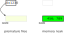
\includegraphics[width=0.4\textwidth]{out/pdf/svg/poitners.pdf}
  \end{center}

\item<2-> $\Rightarrow$ \ao{Garbage collection (GC)}
  \begin{itemize}
  \item \ao{ratain memory block for objects if they could ever be accessed in future
      and reclaim otherwise}
  \item the system automatically does that
  \item $\Rightarrow$ eliminate memory leak and corruption
  \end{itemize}
\item<3-> \ao{the question:} how does the system know
  \ao{\it which objects may be accessed in future}?
\end{itemize}
\end{frame}
\fi

%%%%%%%%%%%%%%%%%%%%%%%%%%%%%%%%%%
\ifja
\begin{frame}[fragile]
\frametitle{今後アクセスされ\{得る・得ない\}もの}
\begin{columns}
\begin{column}{0.6\textwidth}
\begin{itemize}
\item 正確な判定は決定不能
\item ({\tt f(x)}開始時点で)
「{\tt p}が指している領域は今後アクセスされる」
$\iff$
「{\tt f(x)}が終了して0を返す」
$\rightarrow$ 停止問題を解く必要が\ldots

\item $\rightarrow$「今後アクセスされるかも」を大きめに評価
  \begin{itemize}
  \item \aka{NG:} 実はアクセスされるものを回収
  \item \ao{OK:} 実はアクセスされないものを回収しない
  \end{itemize}

\item 上の例ならば{\tt p}はアクセスされる「かも」
($\rightarrow$回収しない)とわかれば十分
\end{itemize}
\end{column}

\begin{column}{0.35\textwidth}
\begin{lstlisting}
int main() {
  if (f(x) == 0) {
    printf("%d\n", p->f->x);
  }    
}
\end{lstlisting}
\begin{center}
%\includegraphics[width=0.6\textwidth]{out/pdf/img/1354150858.pdf}    
\end{center}
\end{column}
\end{columns}
\end{frame}
\fi
%%% END %%%
\ifeng
\begin{frame}[fragile]
\frametitle{Objects that may \{ever/never\} be accessed}
\begin{itemize}
\item the precise judgment is undecidable
\end{itemize}
\begin{columns}
\begin{column}{0.6\textwidth}
\begin{itemize}
\item (at the start of line 2)
``the object pointed to by {\tt p} will ever be accessed''
$\iff$
``{\tt f(x)} will terminate and return 0''
$\rightarrow$ you need to be able to solve the halting problem\ldots
\end{itemize}
\end{column}

\begin{column}{0.35\textwidth}
\begin{lstlisting}
int main() {
  if (f(x) == 0) {
    printf("%d\n", p->f->x);
  }    
}
\end{lstlisting}
\begin{center}
%\includegraphics[width=0.6\textwidth]{out/pdf/img/1354150858.pdf}    
\end{center}
\end{column}
\end{columns}

\begin{itemize}
\item $\rightarrow$ \ao{\it conservatively}
  estimate objects that \ao{\it may be} accessed in future
  \begin{itemize}
  \item \aka{NEVER} reclaim those that are accessed
  \item \ao{OK} not to reclaim those that are in fact never accessed
  \end{itemize}

\item in the above example, OK to retain objects pointed to by {\tt p}
  when the line 2 is about to start
\end{itemize}
\end{frame}
\fi

%%%%%%%%%%%%%%%%%%%%%%%%%%%%%%%%%%
\ifja
\begin{frame}[fragile]
\frametitle{アクセスされる「かも」しれないデータ}
{\small
\begin{itemize}
\item \aka{大域変数}
\item 現在活性な(始まったが終了していない)
  関数呼び出しの\aka{局所変数}
\item<2->\ore{それらからポインタをたどって辿り着くデータ}
\end{itemize}}

\begin{columns}
\begin{column}{0.25\textwidth}
\begin{lstlisting}[]
int * @\aka{\tt s}@;
int * @\aka{\tt t}@;
void h() { ... }
void g() {
  ... 
  h();
  ... = @\aka{\tt p}@->x ...  }
void f() {
  ... 
  g()
  ... = @\aka{\tt q}@->y ... }
int main() {
  ... 
  f()
  ... = @\aka{\tt r}@->z ... }
\end{lstlisting}
\end{column}

\begin{column}{0.65\textwidth}
\begin{center}
\only<1>{\includegraphics[width=\textwidth]{out/pdf/svg/gc_basic_0.pdf}}%
\only<2>{\includegraphics[width=\textwidth]{out/pdf/svg/gc_basic_3.pdf}}
\end{center}
\end{column}
\end{columns}
\end{frame}
\fi
%%% END %%%
\ifeng
\begin{frame}[fragile]
\frametitle{Objects that ``may be'' accessed}
{\small
\begin{itemize}
\item \ao{global variables}
\item \aka{local variables} of
  active function calls (calls that have started but have not finished)
\item<2->\ore{objects reachable from them by traversing pointers}
\end{itemize}}

\begin{columns}
\begin{column}{0.35\textwidth}
  \begin{itemize}
  \item []
\begin{lstlisting}[]
int * @\ao{\tt s}@, * @\ao{\tt t}@;
void h() { ... }
void g() {
  ... 
  h();
  ... = @\aka{\tt p}@->x ...  }
void f() {
  ... 
  g()
  ... = @\aka{\tt q}@->y ... }
int main() {
  ... 
  f()
  ... = @\aka{\tt r}@->z ... }
\end{lstlisting}
\end{itemize}
\end{column}

\begin{column}{0.65\textwidth}
\begin{center}
\only<1>{\includegraphics[width=0.8\textwidth]{out/pdf/svg/gc_basic_0.pdf}}%
\only<2>{\includegraphics[width=0.8\textwidth]{out/pdf/svg/gc_basic_3.pdf}}
\end{center}
\end{column}
\end{columns}
\end{frame}
\fi

%%%%%%%%%%%%%%%%%%%%%%%%%%%%%%%%%%
\ifja
\section{基本原理と用語}
\fi
\ifeng
\section{Basics and Terminologies}
\fi
%%%%%%%%%%%%%%%%%%%%%%%%%%%%%%%%%% 
%%%%%%%%%%%%%%%%%%%%%%%%%%%%%%%%%%
\ifja
\begin{frame}
\frametitle{GCの基本原理(と用語)}
\begin{itemize}
\item \ao{オブジェクト:} メモリ割り当て・回収の単位(Cならばmalloc)
\item \ao{ルート:}
  大域変数や現在活性中の関数の局所変数など,
  ポインタをひとつもたどらずにアクセスされうるオブジェクト
\item \ao{到達可能(reachable):}
  ポインタをたどってたどりつける
\item \ao{生きている(live),死んでいる(dead):}
  今後アクセスされうる,され得ない
\item \ao{ゴミ:} 死んでいるオブジェクト
\item \ao{collector:} GCをするプログラム(やスレッド/プロセス)
\item \ao{mutator:} 要するにユーザプログラムのこと(vs. collector).
  超GC目線な言葉. ユーザプログラムは「グラフを書き換える(mutateする)人」
\end{itemize}
\begin{columns}
\begin{column}{0.8\textwidth}
\begin{beamercolorbox}{ex}
\vskip0.5cm
GCの基本原理: \\
\ao{ルートから到達不能なオブジェクトは死んでいる}
\vskip0.5cm
\end{beamercolorbox}
\end{column}
\begin{column}{0.2\textwidth}
\begin{center}
%\includegraphics[width=0.8\textwidth]{out/pdf/img/1354150858.pdf}
\end{center}
\end{column}
\end{columns}
\end{frame}
\fi
%%% END %%%
\ifeng
\begin{frame}
\frametitle{The basic workings (and terminologies) of GC}
\begin{itemize}
\item<1-> \ao{an object:} the unit of automatic memory allocation/release
  (malloc in C; objects in Java; etc.)
\item<2-> \ao{the root:}
  objects accessible without traversing pointers, such as
  global variables and local variables of active function calls
\item<3-> \ao{reachable objects:} objects reachable from the root
  by traversing pointers
\item<4-> \ao{live / dead objects:}
  objects that \{may be / never be\} accessed in future 
\item<5-> \ao{garbage:} dead objects
\item<6-> \ao{collector:} the program (or the thread/process) doing GC
\item<7-> \ao{mutator:} the user program (vs. collector).
  very GC-centric terminology, viewing the user program
  as someone simply ``mutating'' the graph of objects
\end{itemize}
\begin{center}
  \begin{columns}
    \begin{column}{0.7\textwidth}
\only<8->{      
\begin{beamercolorbox}{ex}
\vskip0.1cm
the basic principle of GC: \\
\ao{objects unreachable from the root are dead}
\vskip0.1cm
\end{beamercolorbox}}
    \end{column}
  \end{columns}
    \end{center}
\end{frame}
\fi

%%%%%%%%%%%%%%%%%%%%%%%%%%%%%%%%%%
\ifja
\section{2大方式}
\fi
\ifeng
\section{Two basic methods}
\fi
%%%%%%%%%%%%%%%%%%%%%%%%%%%%%%%%%% 
%%%%%%%%%%%%%%%%%%%%%%%%%%%%%%%%%%
\ifja
\begin{frame}
\frametitle{2大GC方式}
\begin{itemize}
\item \ao{走査型GC (traversing GC):}
  \begin{itemize}
  \item 素直にルートからポインタをたどり,
    \mura{ルートから到達可能}なオブジェクトを発見
  \item \mura{発見されなかったものを回収}
  \item 2タイプの走査型GC
    \begin{itemize}
    \item \ao{マーク\&スイープGC (mark\&sweep GC)}
    \item \ao{コピーGC (copying GC)}
    \end{itemize}
  \end{itemize}
\item \ao{参照カウントGC (reference counting GC):}
  \begin{itemize}
  \item あるオブジェクトを指すポインタの数\mura{(参照数)を数えながら実行}
  \item \mura{参照数が0になったものを回収}
  \item 注: 参照数が0 $\rightarrow$ 到達不能
  \end{itemize}
\item 注: 巷では走査型GCだけをGCと呼ぶこともあるよう
\end{itemize}
\end{frame}
\fi
%%% END %%%
\ifeng
\begin{frame}
\frametitle{The two major GC methods}
\begin{itemize}
\item \ao{traversing GC:}
  \begin{itemize}
  \item simply traverse pointers from the root, to find (or {\it visit})
    objects \mura{reachable from the root}
  \item \mura{reclaim objects not visited}
  \item two basic traversing methods 
    \begin{itemize}
    \item \ao{mark\&sweep GC}
    \item \ao{copying GC}
    \end{itemize}
  \end{itemize}
\item \ao{reference counting GC (or RC):}
  \begin{itemize}
  \item during execution,
    \mura{maintain the number of pointers (reference count)}
    pointing to each object 
  \item \mura{reclaim an object when its reference count drops to zero}
  \item note: an object's reference count is zero
    $\rightarrow$ it's unreachable from the root
  \end{itemize}
\item remark: ``GC'' sometimes narrowly refers to traversing GC
\end{itemize}
\end{frame}
\fi

%%%%%%%%%%%%%%%%%%%%%%%%%%%%%%%%%%
\ifja
\subsection{走査型GC}
\fi
\ifeng
\subsection{Traversing GC}
\fi
%%%%%%%%%%%%%%%%%%%%%%%%%%%%%%%%%% 
%%%%%%%%%%%%%%%%%%%%%%%%%%%%%%%%%% 
\ifja
\begin{frame}
\frametitle{走査型GCの原理}
\begin{itemize}
\item ルートからポインタをたどっていく
\item これ以上たどるポインタがなくなったところで,
  訪問されていないオブジェクトがゴミ
\item マーク\&スイープとコピーの違いは後述
\end{itemize}

\begin{center}
\only<1>{\includegraphics[width=0.7\textwidth]{out/pdf/lsvg/ms_working_1.pdf}}%
\only<2>{\includegraphics[width=0.7\textwidth]{out/pdf/lsvg/ms_working_2.pdf}}%
\only<3>{\includegraphics[width=0.7\textwidth]{out/pdf/lsvg/ms_working_3.pdf}}%
\only<4>{\includegraphics[width=0.7\textwidth]{out/pdf/lsvg/ms_working_4.pdf}}%
\only<5>{\includegraphics[width=0.7\textwidth]{out/pdf/lsvg/ms_working_5.pdf}}%
\only<6>{\includegraphics[width=0.7\textwidth]{out/pdf/lsvg/ms_working_6.pdf}}
\end{center}
\end{frame}
\fi
%%% END %%%
\ifeng
\begin{frame}
\frametitle{How traversing GC works}
\begin{itemize}
\item traverse pointers from the root
\item once all pointers have been traversed,
  objects that have not been visited are garbage
\item the difference between mark\&sweep and copying is covered later
\end{itemize}

\begin{center}
\only<1>{\includegraphics[width=0.7\textwidth]{out/pdf/lsvg/ms_working_1.pdf}}%
\only<2>{\includegraphics[width=0.7\textwidth]{out/pdf/lsvg/ms_working_2.pdf}}%
\only<3>{\includegraphics[width=0.7\textwidth]{out/pdf/lsvg/ms_working_3.pdf}}%
\only<4>{\includegraphics[width=0.7\textwidth]{out/pdf/lsvg/ms_working_4.pdf}}%
\only<5>{\includegraphics[width=0.7\textwidth]{out/pdf/lsvg/ms_working_5.pdf}}%
\only<6>{\includegraphics[width=0.7\textwidth]{out/pdf/lsvg/ms_working_6.pdf}}
\end{center}
\end{frame}
\fi

%%%%%%%%%%%%%%%%%%%%%%%%%%%%%%%%%%
\ifja
\subsection{参照カウント}
\fi
\ifeng
\subsection{Reference Counting}
\fi
%%%%%%%%%%%%%%%%%%%%%%%%%%%%%%%%%% 
%%%%%%%%%%%%%%%%%%%%%%%%%%%%%%%%%%
\ifja
\begin{frame}[fragile]
\frametitle{参照カウントGCの原理}
\begin{itemize}
\item 各オブジェクトに参照数(それを指すポインタの数)を付随
\item ポインタの書き換え時に参照数更新; $\aka{\tt p} = \ao{\tt q};$を実行
$\rightarrow$
  \begin{itemize}
  \item \aka{\tt p}に入っていたポインタが指すオブジェクトの参照数: 1減る
  \item \ao{\tt q}に入っているポインタが指すオブジェクトの参照数: 1増える
  \end{itemize}
\item 参照数0になったものを回収
$\rightarrow$
回収されたオブジェクト内のポインタが指していたオブジェクトの参照数が1減る
\end{itemize}

\begin{center}
\only<1>{\includegraphics[width=0.7\textwidth]{out/pdf/lsvg/rc_working_1.pdf}}%
\only<2>{\includegraphics[width=0.7\textwidth]{out/pdf/lsvg/rc_working_2.pdf}}%
\only<3>{\includegraphics[width=0.7\textwidth]{out/pdf/lsvg/rc_working_3.pdf}}%
\only<4>{\includegraphics[width=0.7\textwidth]{out/pdf/lsvg/rc_working_4.pdf}}%
\only<5>{\includegraphics[width=0.7\textwidth]{out/pdf/lsvg/rc_working_5.pdf}}
\end{center}
\end{frame}
\fi
%%% END %%%
\ifeng
\begin{frame}[fragile]
\frametitle{How reference counting works}
\begin{itemize}
\item each object has a reference count (RC)
\item update RCs during execution;
  e.g., upon $\aka{\tt p} = \ao{\tt q};$
$\rightarrow$
  \begin{itemize}
  \item the RC of the object \aka{\tt p} points to {\tt -=} 1
  \item the RC of the object \ao{\tt q} points to {\tt +=} 1
  \end{itemize}
\item reclaim an object when its RC drops to zero
  $\rightarrow$
  RCs of objects pointed to by the now reclaimed object
  decrease
\end{itemize}

\begin{center}
\only<1>{\includegraphics[width=0.7\textwidth]{out/pdf/lsvg/rc_working_1.pdf}}%
\only<2>{\includegraphics[width=0.7\textwidth]{out/pdf/lsvg/rc_working_2.pdf}}%
\only<3>{\includegraphics[width=0.7\textwidth]{out/pdf/lsvg/rc_working_3.pdf}}%
\only<4>{\includegraphics[width=0.7\textwidth]{out/pdf/lsvg/rc_working_4.pdf}}%
\only<5>{\includegraphics[width=0.7\textwidth]{out/pdf/lsvg/rc_working_5.pdf}}
\end{center}
\end{frame}
\fi


%%%%%%%%%%%%%%%%%%%%%%%%%%%%%%%%%%
\ifja
\begin{frame}[fragile]
\frametitle{参照数が変化するのは}
\begin{itemize}
\item pointer update {\tt p = q;} {\tt p->f = q;} etc.
\item variables go out of scope
  
\end{itemize}
\end{frame}
\fi
%%% ENG %%%
\ifeng
\begin{frame}[fragile]
\frametitle{When an RC changes}
\begin{itemize}
\item a pointer is updated {\tt \aka{p} = \ao{q};} {\tt \aka{p->f} = \ao{q};} etc.
\item a function gets called
\begin{lstlisting}
int main() {
  object * q = ...;
  f(@\ao{\tt q}@);
}
\end{lstlisting}
\item a variable goes out of scope or a function returns
\begin{lstlisting}
f(object * p) {
  ...  
  {
    object * r = ...;

  } /* RC of @\aka{\tt r}@ should decrease */
  ...
  return ...; /* RC of @\aka{\tt p}@ should decrease */
}    
\end{lstlisting}
\item etc. any point pointer variables get copied / become no longer used
\end{itemize}
\end{frame}
\fi
%%%%%%%%%%%%%%%%%%%%%%%%%%%%%%%%%%

%%%%%%%%%%%
\ifja
\begin{frame}
  \frametitle{日本語タイトル}
  \begin{itemize}
  \item あ
  \end{itemize}
\end{frame}
\fi
%%% ENG %%%
\ifeng
\begin{frame}
  \frametitle{Shortcomings of GC}
  \begin{itemize}
  \item may be \mura{costly}
    \begin{itemize}
    \item what if a traversing GC visits 10GB of reachable objects,
      to reclaim only 100MB of memory?
    \end{itemize}
  \item may \mura{pause the user program (mutator) for a long time}
    \begin{itemize}
    \item a traversing GC does not want the mutator to modify the
      object graph while traversing it
    \end{itemize}
  \item may \mura{slow the user program}
    \begin{itemize}
    \item esp. by reference counting
    \end{itemize}
  \end{itemize}
  
  methods to overcome some of the issues
  will be covered in later weeks
\end{frame}
\fi
%%%%%%%%%%%

\end{document}

